\documentclass[12pt]{article}
\usepackage{amssymb,amsfonts,amsmath,graphicx,mathtools}
\usepackage[alphabetic,y2k,lite]{amsrefs}
\usepackage{fullpage, mystyle}
\usepackage{MnSymbol}
\usepackage{tikz}
\usepackage{tikz-cd}

\tikzset{
small_morphism/.style={fill=white,circle,draw=white,thin,inner sep=1pt, minimum size=10pt, scale=0.8},
dotnode/.style={fill=black,circle,minimum size=2.5pt, inner sep=1pt, outer sep=0},
}

\newcommand{\cB}{{\mathcal{B}}}
\newcommand{\cD}{{\mathcal{D}}}
\newcommand{\Mod}{{\mathcal{M}\textrm{od}}}
\newcommand{\cHom}{{\mathcal{H}\text{om}}}
\newcommand{\cFun}{{\mathcal{F}un}}
\newcommand{\Vect}{{\textrm{Vec}}}
\newcommand{\bigboxplus}{\Huge \boxplus}

\newcommand{\bimod}[2]{{#1\textrm{-bimod-}#2}}
\newcommand{\amod}[1]{{#1\textrm{-mod}}}
\newcommand{\moda}[1]{{\textrm{mod-}#1}}
\newcommand{\ModA}[1]{{\Mod(#1)}}


\begin{document}

\title{Note in preparation for talk for seminar on Fusion 2-Categories, Winter semester 2022, UHH}
\author{Ying Hong Tham}
\date{28 December, 2022}
\maketitle

[Almost everything here is from \cite{DRfusion};
the only things that are new here are
cleaner proofs of the main theorems
as suggest by David Reutter.]


The main goal of thie note is to prove that
a finite semisimple 2-category is the
category of finite semisimple modules
over a multifusion category, and vice versa.


That is, for a semisimple 2-category $\cC$,
there exists a multifusion category $C$
such that

\[
\cC \simeq \Mod_{s.s.}^{fin}(C)
\]

Here $\Mod_{s.s.}^{fin}(C)$,
which we will abbreviate to $\ModA{C}$,
stands for finite semisimple right module categories over $C$.

Conversely, for any mutifusion category $C$,
$\ModA{C}$ is a finite semisimple 2-category.



\subsection{Conventions}

Everything is over an algebraically closed field $\kk$
with characteristic 0.

We use different fonts/alphabets for different levels
of structures:

In relation to a 2-category:
\begin{itemize}
\item $\cC$ (caligraphic font): 2-category;

\item $X,Y,F$ (upper case latin): object of 2-category,
	functor between 2-categories;

\item $f,g$ (lower case latin): 1-morphism;
	we write $\cC(X,Y)$ for the category of morphisms
	from $X$ to $Y$;

\item $\eta,\veps,\delta$ (lower case greek): 2-morphism;
	for a 2-morphism $\alpha: f \Rightarrow g: X \to Y$,
	we may write $\alpha \in \cC(X,Y)(f,g)$
	to indicate its sources and targets,
	or simply $\alpha \in \Hom(f,g)$ if the objects are clear
\end{itemize}

In relation to a 1-category:
\begin{itemize}
\item $C,A$ (upper case latin): category;

\item $a,b,f,g$ (lower case latin): objects in category,
	functor between categories;

\item $\alpha,\beta$ (lower case greek): morphism in category
\end{itemize}

[We use the same type of font for 1-functors and 1-morphisms
because the 1-morphisms in the 2-category $\Mod(C)$
of module categories are module functors,
and we want the notation to be consistent;
we use the same type of font for 2-functors and objects
because 2-functors are objects in the 2-category of
2-functors]

We also compose morphisms from right to left:
in a 2-category $\cC$,
for $\alpha \in \cC(X,Y)(f,f'),
\beta \in \cC(Y,Z)(g,g'),
\gamma \in \cC(X,Y)(f',f'')$,
we write
\[
g \circ f, g \circ f', \ldots : X \to Z
\]
for composition of 1-morphisms,
\[
\beta \circ \alpha: (g \circ f) \Rightarrow (g' \circ f'):
	X \to Z
\]
for horizontal composition of 2-morphisms,
\[
\gamma \cdot \alpha: f \Rightarrow f'' : X \to Y
\]
for vertical composition of 2-morphisms.


We may also omit the composition symbols
if the type of composition is clear
(in particular for composition of 1-morphisms).



In general, if $P$ is a property of a 1-category,
we say that a 2-category $\cC$ is \emph{locally $P$}
if every hom-category $\cC(X,Y)$ satisfies $P$.

By 2-category we always mean a weak 2-category
that is furthermore locally additive over $\kk$,
that is, all hom-categories are
additive categories over $\kk$,
and all compositions are $\kk$-bilinear.
By 2-functor (sometimes just functor for simplicity)
between 2-categories will always be locally $\kk$-linear.


\section{Review}

Let us recall some definitions and facts concerning
semisimple 2-categories.
These where covered in more detail in previous talks,
so here we will simply state them without proof.

\subsection{Additive 2-category, direct sums of objects}

\begin{definition}[direct sum of objects in 2-category]
A \emph{direct sum} of two objects $A_1,A_2$ in $\cC$
is an object $A_1 \boxplus A_2$ together with
inclusion and projection 1-morphisms
$i_k : A_k \rightleftharpoons A_1 \boxplus A_2 : p_k$,
such that
\begin{itemize}
\item $p_k \circ i_k \simeq \id_{A_k}$,
\item $p_2 \circ i_1$, $p_1 \circ i_2$ are zero 1-morphisms,
\item $\id_{A_1 \boxplus A_2} \simeq
	i_1 \circ p_1 \oplus i_2 \circ p_2$
\end{itemize}
\end{definition}

\begin{proposition}
$i_k,p_k$ are two-sided adjoints to each other.
\end{proposition}


\begin{definition}
A 1-morphism $i: X \to Y$ is \emph{fully faithful}
(or $(X,i)$ is a \emph{subobject} of $Y$)
if it induces fully faithful functors between hom-categories
by post-composition, i.e. for all objects $A$,
$i \circ - : \cC(A,X) \to \cC(A,Y)$
is fully faithful.
\end{definition}

\begin{proposition}
$i_k: A_k \to A_1 \boxplus A_2$ is fully faithful.
\end{proposition}



(I don't think the following was discussed,
but it is a simple concept anyway)

\begin{definition}[Direct sum of 2-categories]
Given 2-categories $\cC_j$, $j \in J$,
we may consider the direct sum 2-category
$\cC := \bigboxplus_{j \in J} \cC_j$:
\begin{itemize}
\item $\Obj \cC = \bigsqcup_{j \in J} \Obj \cC_j$

\item for $X \in \cC_i, Y \in \cC_j$,
	$\cC(X,Y) =
\begin{cases}
	\cC_j(X,Y) \;\; \text{if } i = j
	\\
	0 \;\; \text{if } i \neq j
\end{cases}
$
\end{itemize}
\end{definition}

\subsection{Idempotent completeness, separable monads, splittings}

\begin{definition}
A \emph{separable algebra} $(a,\mu,\eta)$ in a tensor category $C$
is an algebra that admits an $a$-$a$-bimodule section
$\prescript{}{a}a_a \to \prescript{}{a}a \tnsr a_a$
to $\mu$.
\end{definition}

\begin{definition}
Let $(t, \mu, \eta)$ be a monad on an object $X$
in a 2-category $\cC$.
We say $t$ is \emph{separable} if there is a
$t$-$t$-bimodule section
$t \Rightarrow t \circ t$ to $\mu$.
\end{definition}

In other words, a separable monad over $X$
is a separable algebra in $\cC(X,X)$.

\begin{definition}
Let $r \vdash l: X \to Y$ be an adjunction
with unit $\eta: \id_X \Rightarrow rl$
and counit $\veps: lr \Rightarrow \id_Y$.
We say the adjunction $l \dashv r$ is \emph{separable}
if $\veps$ admits a section.
\end{definition}

Clearly, if an adjunction $l \dashv r$ is separable,
then the monad $rl$ is separable.

\begin{definition}
Let $(t,\mu,\eta)$ be a separable monad on
an object $X \in \cC$.
A \emph{(separable) splitting} of $t$ is a (separable) adjunction
$r \vdash l: X \to Y$
together with an isomorphism
$\psi: rl \simeq t$ as monads on $X$.
\end{definition}

Under the right conditions
(local idempotent completeness of $\cC$),
splittings are unique (see \prpref{p:splitting-unique}).


\begin{proposition}[Uniqueness of splitting]
[\cite{DRfusion}, Theorem A.3.1]
\label{p:splitting-unique}
In a locally idempotent complete 2-category $\cC$,
splittings of a separable monad are unique
up to equivalence.
\end{proposition}

In particular, this holds true when $\cC$
is locally semisimple.

Thought to self:
\cite{DRfusion} proves this by showing that
a splitting is equivalent
to an ``Eilenberg-Moore object'' and also a ``Kleisli object'',
which are in themselves important and interesting objects
characterized by universal properties.
I'd like to have a more direct proof,
somehow constructing an equivalence between any two splittings
directly from the splitting data.
I don't have a full proof, but here's an attempt.
Say for a separable monad $t$ on $X$,
we have two adjunctions $r \vdash l : X \to Y$
and $r' \vdash l' : X \to Y'$
that split $t$.
There is are obvious 1-morphisms $l' \circ r: Y \to Y'$,
$l \circ r': Y' \to Y$,
but it is unlikely that these are equivalences.
A promising candidate for an equivalence
is $l' \circ_t r$, the coequalizer of
$l' \circ t \circ r \Rightarrow l' \circ r$
(here $r$ is a left $t$-module from the counit:
$tr \simeq rlr \Rightarrow r$;
similarly $l'$ is a right $t$-module).
Such a coequalizer does appear in the proof of
\cite{DRfusion}*{Theorem A.3.1} anyway,
and I've found that this thought process
makes the consideration of the Eilenberg-Moore and Kleisli
objects more motivated.


Now that we've defined the notion on objects,
we consider the property as a global 2-category-wide property:


\begin{definition}
A 2-category $\cC$ is \emph{idempotent complete}
if every separable monad admits a splitting.
\end{definition}

\begin{definition}
Let $\cC$ be a locally idempotent complete 2-category.
Define the \emph{idempotent completion of $\cC$},
denoted $\cC^\nabla$, to be the 2-category whose objects
are given by separable monads of $\cC$,
and the hom-category of morphisms from
separable monad $(X,p)$ to $(Y,q)$
is the category $\bimod{q}{p}(\cC(X,Y))$
of $q$-$p$-bimodules in $\cC(X,Y)$.

There is a natural 2-functor $I: \cC \to \cC^\nabla$
that is fully faithful.

A 2-functor $F: \cC \to \cD$
extends to a 2-functor $F^\nabla: \cC^\nabla \to \cD^\nabla$
that commutes with $I$'s.
\end{definition}


\begin{proposition}
$\cC^\nabla$ is idempotent complete.
Moreover, if $\cC$ is already idempotent complete,
then $I: \cC \simeq \cC^\nabla$ is an equivalence.
\end{proposition}

As a consequence, if $\cD$ is idempotent complete,
then we have equivalences of 2-categories
\[
\cFun(\cC,\cD) \simeq \cFun(\cC^\nabla,\cD^\nabla)
\simeq \cFun(\cC^\nabla, \cD)
\]

\begin{proposition}
If $F: \cC \to \cD$ is fully faithful,
then $F^\nabla: \cC^\nabla \to \cD^\nabla$
is also fully faithful.
\end{proposition}



$(-)^\nabla$ is a categorified version of the
Karoubi completion operation.
By going along the lines of \cite{Ostrik},
the definition of $\cC^\nabla$
is very suggestive of the idea that
objects of $\cC^\nabla$ should be thought of as
the Morita 2-category of algebras in some tensor category;
indeed, let $C$ be multifusion,
and let $\cB C$ be the 2-category with one object $*$
and endmorphisms given by $C$
(the ``delooping of $C$'').
Then by construction, we have
\[
(\cB C)^\nabla =
\begin{cases}
	\Obj: \text{ separable algebras in } C
	\\
	\text{Mor}: (\cB C)^\nabla (a,b) = \bimod{b}{a}(C)
\end{cases}
\]


\begin{proposition}[\cite{DRfusion}*{Prop 1.3.13}]
\label{p:modC-deloop}
For a multifusion category $C$,
the following 2-functor is an equivalence:
\[
\begin{tikzcd}[row sep = tiny]
\amod{(-)}(C) :
	& (\cB C)^\nabla
	\ar[r]
	& \ModA{C}
\\
\Obj:
	& a
	\ar[r,mapsto]
	& \amod{a}(C)
\\
1\textrm{-Mor}:
	& \prescript{}{b}m_a
	\ar[r,mapsto]
	& m \tnsr_a -
\\
2\textrm{-Mor}:
	& \vphi
	\ar[r,mapsto]
	& \vphi \tnsr_a -
\end{tikzcd}
\]
\end{proposition}

\begin{proof}
Essential surjectivity follows from:\\
-\cite{Ostrik}*{Theorem 1}: for a finite semisimple right module
category over multifusion $C$, there exists a semisimple algebra
$a$ in $C$ such that $M \simeq \amod{a}(C)$
as right $C$-module categories; and\\
-\cite{DSPSb}*{Corollary 2.6.9}: When $C$ is multifusion over
a field of characterisitc 0,
a right $C$-module category $M$ is separable
($\simeq \amod{a}(C)$ for a separable algebra $a$)
if and only if it is semisimple.

Fully faithfulness follows from \cite{EGNO}*{Prop 7.11.1}.
\end{proof}

This is almost one half of the main result;
one still needs to prove local semisimplicity
and existence of adjoints.
This will follow from more results from \cite{DSPSa},\cite{DSPSb},
which we show later.




\subsection{Simple objects}


\begin{proposition}[equivalent notions of simple-ness]
Let $\cC$ be a locally finite semisimple and
idempotent complete 2-category,
and let $X \in \cC$ be a nonzero object.
Then the following notions of $X$ being simple are equivalent:

(1) any subobject $i: Y \to X$ of $X$
 is either 0 ($Y \simeq 0$)
 or ($i$ is) an equivalence;

(2) $X$ cannot be written as a non-trivial direct sum,
	i.e. if $X = \boxplus X_i$,
	then $X_i \simeq 0$ for all but one $i$;

(3) $\id_X$ is a simple object in $\cC(X,X)$.
\end{proposition}

\begin{proof}[Proof idea]
(1) $\Rightarrow$ (2): Contravariant statement
follows from fully faithfulness of
$i_k: A_k \to A_1 \boxplus A_2$.

(2) $\Rightarrow$ (3): Contravariant statement is
``identity splitting implies object splitting'',
uses idempotent completeness of $\cC$
to split out objects corresponding to summands of $\id_X$
(which are separable monads)
(see \cite{DRfusion}*{Prop 1.3.16}).

(3) $\Rightarrow$ (1): for non-zero fully faithful $r: Y \to X$,
with $\id_X$ simple,
consider the left adjoint $l: X \to Y$,
use fully faithfulness to get a preimage
$\delta : \id_Y \Rightarrow lr$ of
$\eta \circ r: r \Rightarrow rlr$.
Use simplicity of $\id_X$ to get section of the unit $\eta$.
Show $\delta$ is a section of the counit. Etc.
(See \cite{DRfusion}*{Prop 1.2.14})
\end{proof}


\subsection{Semisimple 2-category}

\begin{definition}[(finite) semisimple 2-category]
A 2-category $\cC$ is \emph{semisimple}
if it is:
\begin{itemize}
\item locally semisimple,
\item admits left and right adjoints for every 1-morphism,
\item additive,
\item idempotent complete.
\end{itemize}

It is furthermore \emph{finite semisimple}
if it is also locally finite and
has finitely many equivalence classes of simple objects.
\end{definition}


%%%%%%%%%%%%%%%%%%%%%%%%%%%%%%%%%%%%%%%%%%%%%%%%%%%%%%%%%%%%%%
\section{New stuff}

Beyond this point, we cover new stuff
(i.e. not covered in previous talks).

\subsection{Schur's lemma}

The equivalence between notions of a simple object
in a seimsimple 2-category,
as we just recalled,
is quite similar to the semisimple 1-category case.
However, there is a stark difference in that
there can be nonzero morphisms between
non-equivalent simple objects;
indeed, recall our running example of a 2-category
$\ModA{\Vect_{\ZZ/2}}$:

\[
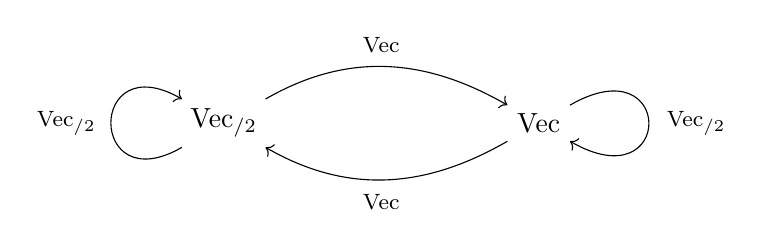
\begin{tikzpicture}
\node (a) at (0,0) {$\Vect_{\ZZ/2}$};
\node (b) at (4,0) {$\Vect$};
\draw[->] (a) to[out=30,in=150] (b);
\node at (2,1) {\footnotesize $\Vect$};
\draw[->] (b) to[out=-150,in=-30] (a);
\node at (2,-1) {\footnotesize $\Vect$};
\draw[->] (a) .. controls +(-150:2cm) and +(150:2cm) .. (a);
\node at (-2,0) {\footnotesize $\Vect_{\ZZ/2}$};
\draw[->] (b) .. controls +(30:2cm) and +(-30:2cm) .. (b);
\node at (6,0) {\footnotesize $\Vect_{\ZZ/2}$};
\end{tikzpicture}
\]


The existence of nonzero 1-morphisms
between non-equivalent simple objects
turns out to be a very important aspect of semisimple 2-categories
since, as we shall see,
it captures 2-Morita equivalences between fusion categories.

\begin{proposition}
[Schur's Lemma, \cite{DRfusion}*{Prop 1.2.19}]
\label{p:schur-lemma}
In a semisimple 2-category $\cC$,
if $f: A \to B, g: B \to C$ are nonzero 1-morphisms
between simple objects $A,B,C$,
then $g \circ f$ is also nonzero.
\end{proposition}

\begin{proof}[Proof of \prpref{p:schur-lemma}]
Let $f^*: B \to A$ be a right adjoint to $f$.
Since $\id_B$ is simple, there exists a section
$\delta: \id_B \Rightarrow ff^*$
to the counit $\veps: ff^* \Rightarrow \id_B$.
Postcomposing with $g$,
we have $\id_g = (\id_g \circ \veps) \cdot (\id_g \circ \delta):
g \Rightarrow gff^* \Rightarrow g$.
Thus if $gf = 0$, then $\id_g = 0$,
contradicting nonzero-ness of $B$.
\end{proof}

Thus, this establishes transitivity on a weaker notion
of equivalence among simple objects
(namely, existence of nonzero 1-morphism);
reflexivity is obvious,
and symmetry is given by adjoints.

\begin{definition}[component of semisimple 2-category]
In a semisimple 2-category $\cC$,
we say two simple objects $A,B$ belong to the same
\emph{component} if there exists a nonzero 1-morphism
$f: A \to B$.
\end{definition}


In a finite semisimple 2-category $\cC$,
there will be finitely many components,
say index by a set $J$.
Consider one component $j \in J$,
and consider the full subcategory $\cC_j$ of $\cC$
consisting of objects that are equivalent
to a direct sum of simples in the component $j$.
Clearly, this gives us a decomposition of $\cC$ into a direct sum
$\cC \simeq \bigboxplus_{j \in J} \cC_j$.


\subsection{Main result}

\begin{theorem}[\cite{DRfusion}*{Theorem 1.4.8}]
The 2-category of finite semisimple module categories
of a multifusion category
is a finite semisimple 2-category.
\end{theorem}

\begin{proof}
Let $C$ be a multifusion category.

From \prpref{p:modC-deloop},
we already see that $\ModA{C} \simeq (\cB C)^\nabla$
is idempotent complete
and locally idempotent complete.
$\ModA{C}$ is clearly already additive.


Locally semisimple-ness follows directly from
\cite{DSPSb}*{Corollary 2.5.6},
and existence of adjoints for 1-morphisms
follows from \cite{DSPSa}*{Corollary 2.13}.

For self understanding, more details of proofs of these two
properties:

Locally semisimple-ness:
One of the main results of \cite{DSPSb} is
Theorem 2.5.5, which states that
the relatie Deligne tensor product
of separable bimodule categories is also separable.
Separable-ness is the stand in for semisimple-ness
for arbitrary fields,
and again by \cite{DSPSb}*{Corollary 2.6.9},
is equivalent to semisimple-ness in our case of
$\text{char }\kk = 0$.
We have, for separable algebras $a,b$,
$\bimod{b}{a}(C) \simeq \amod{b}(C) \boxtimes_{C} \moda{a}(C)$
is separable, hence semisimple.

Existence of adjoints for 1-morphisms:
functors between semisimple 1-categories
are automatically exact,
hence admit both right and left adjoints.
Then the results follows from \cite{DSPSa}*{Corollary 2.13},
which states that the adjoints can be promoted
to respect the bimodule structures.
(As stated in \cite{DSPSa}, it only says there
exists adjoints that respect bimodule structures,
but the proof actually implies more,
that the given adjoint can be promoted.)
\end{proof}


\begin{theorem}[\cite{DRfusion}*{Theorem 1.4.9}]
Every finite semisimple 2-category is equivalent to
the 2-category of finite semisimple module categories
of a multifusion category.
\end{theorem}

\begin{proof}
For simplicity, let us assume that $\cC$ has only one component.
Indeed, if there are multiple components,
then from our previous discussion,
we have a direct sum decomposition
$\cC =\simeq \bigboxplus_{j \in J} \cC_j$,
and if $\cC_j \simeq \ModA{C_j}$ for multifusion $C_j$,
then $\cC \simeq \ModA{\bigoplus_{j \in J} C_j}$.

Take a simple object $X$,
and let $C = \cC(X,X)$.
Since $\id_X$ is simple, $C$ is in fact fusion.

Consider the inclusion 2-functor
\begin{align*}
F : \cB C &\to \cC
\\
* &\mapsto X
\end{align*}
which is fully faithful by construction.
Then
\[
F^\nabla: \cB C \to \cC
\]
is fully faithful.
It remains to show that $F^\nabla$ is essentially surjective,
in particular, that any simple is in the essential image
of $F^\nabla$.

Let $Y$ be a simple object in $\cC$.
Since $\cC$ only has one component,
there exists a nonzero 1-morphism
$f: X \to Y$;
it has a (nonzero) right adjoint $g: Y \to X$,
with counit $\veps : fg \Rightarrow \id_Y$.
Since $Y$ is simple, $\id_Y$ is simple,
so $\veps$ admits a section,
hence $f \dashv g$ is a separable adjunction.
Thus, by uniqueness of separable splittings,
$Y$ is in the essential image of $F^\nabla$.
\end{proof}


In the proof above,
the only property of $X$ that we used is the fact that
there exists a nonzero 1-morphism from $X$ to every simple
in $\cC$,
and thus any $X$ will do.
Taking, say, $X = \boxplus X_i$,
where the sum is over equivalence classes of simples,
would result in a multifusion $C = \cC(X,X)$.

We can also avoid the first step of taking only one component
of $\cC$,
as long as we are careful to take $X$
that has at least one object from each component
in its direct sum decomposition.


\begin{figure}
\centering
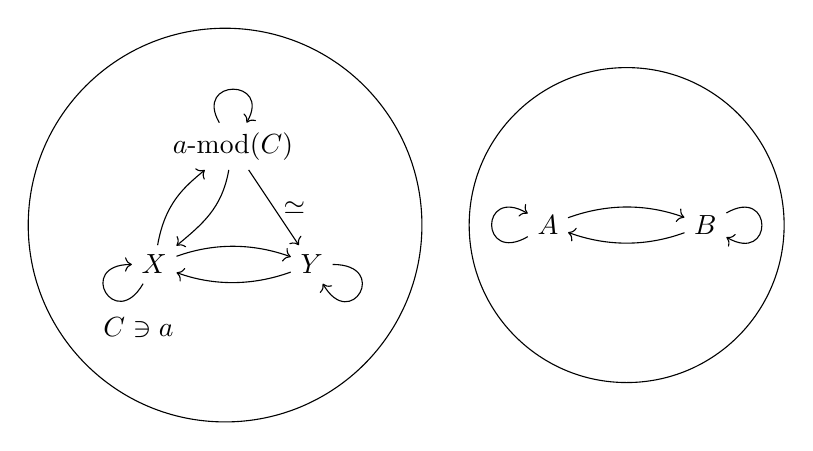
\begin{tikzpicture}
\draw (0.9,0.5) circle (2.5cm);
\node (x) at (0,0) {$X$};
\node (y) at (2,0) {$Y$};
%\node (z) at (1,1.5) {$Z$};
\node (z) at (1,1.5) {$\amod{a}(C)$};
%\node at (0.8,-1.3) {$X \boxplus Y$};
%\node[small_morphism,label={-45:$X$}] (x) at (0,0) {};
%\node[dotnode,label={-45:$Y$}] (y) at (2,0) {};
%\node[dotnode,label={30:$Z$}] (z) at (1,1.5) {};
%%
\draw[->] (x) .. controls +(-120:1cm) and +(180:1cm) .. (x);
\draw[->] (y) .. controls +(0:1cm) and +(-60:1cm) .. (y);
\draw[->] (z) .. controls +(120:1cm) and +(60:1cm) .. (z);
\node at (-0.2,-0.8) {$C \ni a$};
%
\draw[->] (x) .. controls +(20:0.8cm) and +(160:0.8cm) .. (y);
%\draw[->] (y) .. controls +(140:0.8cm) and +(-80:0.8cm) .. (z);
\draw[->] (z) .. controls +(-100:0.8cm) and +(40:0.8cm) .. (x);
%
\draw[->] (y) .. controls +(-160:0.8cm) and +(-20:0.8cm) .. (x);
%\draw[->] (z) .. controls +(-40:0.8cm) and +(100:0.8cm) .. (y);
\draw[->] (z) -- (y)
	node[pos=0.5,right] {$\simeq$};
\draw[->] (x) .. controls +(80:0.8cm) and +(-140:0.8cm) .. (z);
%%%%%%%%%%%%%%%%%%%%%%%%%%%%%
\begin{scope}[shift={(5,0.5)}]
\draw (1,0) circle (2cm);
\node (a) at (0,0) {$A$};
\node (b) at (2,0) {$B$};
%\node at (1.5,1.5) {$A \boxplus B$};
%%
\draw[->] (a) .. controls +(-150:1cm) and +(150:1cm) .. (a);
\draw[->] (b) .. controls +(30:1cm) and +(-30:1cm) .. (b);
%
\draw[->] (a) .. controls +(20:0.8cm) and +(160:0.8cm) .. (b);
\draw[->] (b) .. controls +(-160:0.8cm) and +(-20:0.8cm) .. (a);
\end{scope}
\end{tikzpicture}
\caption{Abstract picture of finite semisimple 2-categories,
showing the simples separated into components;
within each component,
every simple can be recovered from the endomorphism category
of other simples.
}
\end{figure}


\begin{remark}
Every object (assuming $\cC$ has one component)
contains the information need to reconstruct every other object;
given any nonzero $X$,
every object is constructed from the endomorphisms of $X$.

This is reminiscent of the metaphor of
Indra's Net from Mahayana Buddhism,
where, in the realm of the god Indra,
there is a vast net that stretches infinitely in all directions;
at each crossing there is a jewel that perfectly reflects,
and in the reflection is every other jewel,
and within them is again reflected every other jewel and so on.
The metaphor is meant to capture the concept of the
interconnectedness of all phenomena.

A concrete ``picture'' of Indra's Net is the universal cover
of $\mathbf{T}^3 \# \mathbf{T}^3$:
at every lattice point in $\ZZ^3 \subset \RR^3$,
cut out a ball;
at each ball, invert the exterior into itself;
repeat this process infinitely.
\end{remark}


\begin{example}
Consider $C = \Vect_{G}$ for a finite group $G$.
We will focus on two of its algebras,
the trivial algebra $\kk_e$
and the group algebra $\kk[G] = \bigoplus \kk_g$,
which we denote by $e$ and $f$, respectively,
as objects of $C$.

Clearly $\amod{e}(C)$ is simply $C$ itself
as a right module category over itself.
For $r$, it is clear that a module over $r$ in $C$
is determined by any of its components
(as a $G$-graded vector space),
thus $\amod{f}(C) \simeq \Vect$,
with right $C$-module action given by forgeting
the grading on $C$.

Next we study the functor categories.
Clearly the $C$-endofunctors of $C_C$ is $C$ itself.
For $\amod{f}(C)$,
an endofunctor is given by an $f$-$f$-bimodule in $C$.
Let $m \in \bimod{f}{f}(C)$;
write $m = \bigoplus m_g$.
The right $f$-action on $m$ makes all the $m_g$ isomorphic
in a coherent manner.
For $h \in G$, conjugation (left action by $h$ and right action
by $h^\inv$) gives an action of $G$ on $m_e$;
this action completely determines the left action
on other components $m_g$ as well.
Thus, $\ModA{C}(f,f) \simeq \Rep(G)$,
where we simply write $f$ for $\amod{f}(C)$ for simplicity.

For functor categories between them, we see that
$\ModA{C}(e,f) \simeq \bimod{f}{e}(C) \simeq \amod{f}(C)
\simeq \Vect$
and
$\ModA{C}(f,e) \simeq \bimod{e}{f}(C) \simeq \moda{f}(C)
\simeq \Vect$.

Thus we recover the running example of $\ModA{\Vect_{\ZZ/2}}$;
we note that in the simple case of $G = \ZZ/2$,
$\Vect_{\ZZ/2} \simeq \Rep(\ZZ/2)$,
but here we see a difference between the endomorphism
categories of the two objects we considered.


Of course, there are many other algebras.
For a subgroup $H \subseteq G$,
we can consider the group algebra $\kk[H]$,
which we denote by $h$ as an object in $C$.
The category of modules $\amod{h}(C)$
is simply the direct sum $\bigoplus_{H \backslash G} \Vect$,
as the components $m_g$ of an $h$-module
must be the same within each $H$-orbit.
The endomorphism category seems a lot more complicated.
\end{example}



\begin{thebibliography}{1}

\bibitem{DRfusion} Douglas, Christopher L., and David J. Reutter. ``Fusion
2-categories and a state-sum invariant for 4-manifolds.'' arXiv preprint arXiv:1812.11933 (2018).

\bibitem{Ostrik} Ostrik, Victor. ``Module categories, weak Hopf algebras and
modular invariants.'' Transformation groups 8, no. 2 (2003): 177-206.

\bibitem{DSPSa} C. L. Douglas, C. Schommer-Pries, and N. Snyder. The balanced tensor product of module
categories. Kyoto J. Math., 2017. arXiv:1406.4204.

\bibitem{DSPSb} C. L. Douglas, C. Schommer-Pries, and N. Snyder. Dualizable tensor categories. Mem. Amer.
Math. Soc., 2017. arXiv:1312.7188.

\bibitem{EGNO} P. Etingof, S. Gelaki, D. Nikshych, and V. Ostrik. Tensor Categories. American Mathematical
Society, 2015. Available online at http://www.math.mit.edu/~etingof/egnobookfinal.pdf.

\end{thebibliography}



\end{document}
